\documentclass[border=1cm]{standalone}

\usepackage{tikz}

\usetikzlibrary{3d,calc}

\begin{document}
    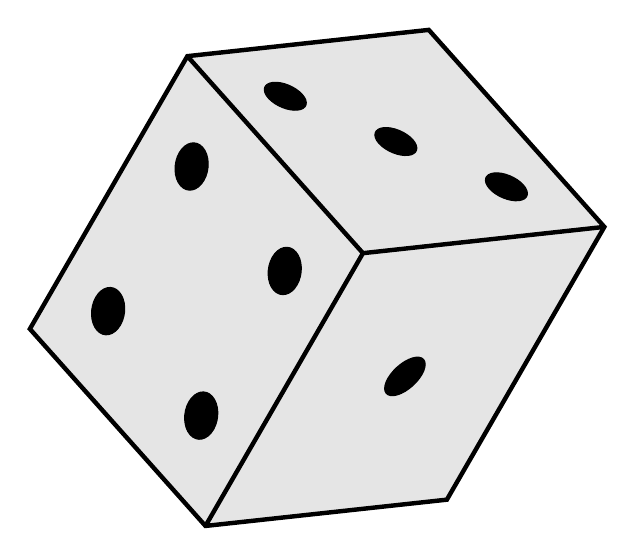
\begin{tikzpicture}
        \begin{scope}[rotate around z=-30, rotate around y=-30]
            \foreach \i in {0,...,3}{
                \coordinate[shift={(0,0,-2)}] (P\i) at (45+90*\i:{2*sqrt(2)});
                \coordinate[shift={(0,0,2)}] (Q\i) at (45+90*\i:{2*sqrt(2)});
            }
            \draw[ultra thick, fill=gray!20] (P0)--(P1)--(Q1)--(Q2)--(Q3)--(P3)--cycle (Q1)--(Q0)--(P0) (Q0)--(Q3);
            \begin{scope}[canvas is zy plane at x=2,fill]
                \draw[fill=black] (0,0) circle (8pt);
            \end{scope}
            \begin{scope}[canvas is xy plane at z=2]
                \draw[fill=black] (45:1.5) circle (8pt);
                \draw[fill=black] (135:1.5) circle (8pt);
                \draw[fill=black] (225:1.5) circle (8pt);
                \draw[fill=black] (315:1.5) circle (8pt);
            \end{scope}
            \begin{scope}[canvas is xz plane at y=2]
                \draw[fill=black] (0,0) circle (8pt);
                \draw[fill=black] (135:1.5) circle (8pt);
                \draw[fill=black] (-45:1.5) circle (8pt);
            \end{scope}
        \end{scope}
    \end{tikzpicture}
\end{document}